\section{Ergebnispräsentation}

\begin{frame}{Kommunikationsprotokoll}
  \vspace{1em}
%   \Large
  \begin{figure}[!ht]
    \centering
    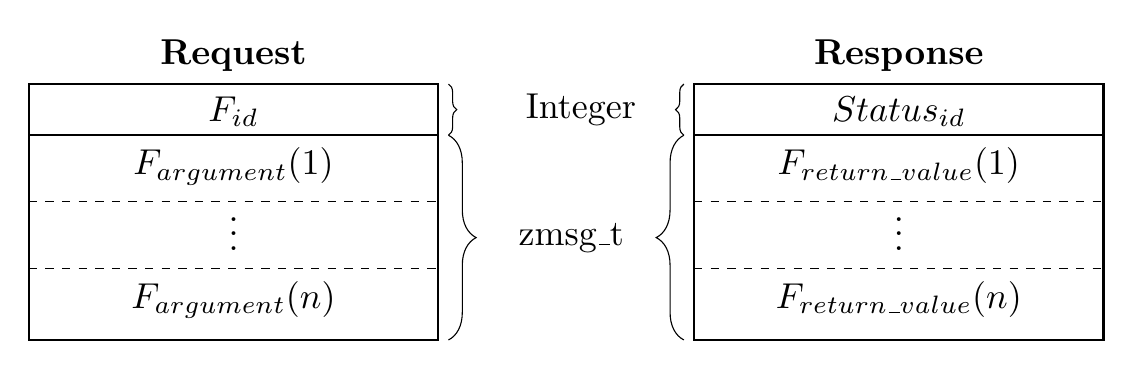
\begin{tikzpicture}[scale=1.3, every node/.style={scale=1.3}]
        % Request box
        \node[above] at (2, 2.5) {\textbf{Request}};
        \draw[thick] (0, 2.5) rectangle (4, 0);
        \node[below] at (2, 2.5) {$F_\text{id}$};
        \draw[thick] (0, 2) -- (4, 2);
        \node[below] at (2, 2) {$F_\text{argument}(1)$};
        \draw[dashed] (0, 1.35) -- (4, 1.35);
        \node[below] at (2, 1.53) {$\vdots$};
        \draw[dashed] (0, 0.7) -- (4, 0.7);
        \node[below] at (2, 0.7) {$F_\text{argument}(n)$};
        \draw[decorate, decoration={brace, amplitude=10pt}] (4.1, 2) -- (4.1, 0)
            node[midway, right=16pt] {\text{zmsg\_t}};
        \draw[decorate, decoration={brace, amplitude=3pt}] (4.1, 2.5) -- (4.1, 2)
            node[midway, right=18pt] {\text{Integer}};
        % Response box
        \node[above] at (8.5, 2.5) {\textbf{Response}};
        \draw[thick] (6.5, 2.5) rectangle (10.5, 0);
        \node[below] at (8.5, 2.5) {$Status_\text{id}$};
        \draw[thick] (6.5, 2) -- (10.5, 2);
        \node[below] at (8.5, 2) {$F_\text{return\_value}(1)$};
        \draw[dashed] (6.5, 1.35) -- (10.5, 1.35);
        \node[below] at (8.5, 1.53) {$\vdots$};
        \draw[dashed] (6.5, 0.7) -- (10.5, 0.7);
        \node[below] at (8.5, 0.7) {$F_\text{return\_value}(n)$};
        \draw[decorate, decoration={brace, amplitude=10pt}] (6.4, 0) -- (6.4, 2);
        \draw[decorate, decoration={brace, amplitude=3pt}] (6.4, 2) -- (6.4, 2.5);

    \end{tikzpicture}
    % \caption{Das Kommunikationsprotokoll zwischen Client und Server.}
    % \label{fig:protocol}
  \end{figure}
\end{frame}

\begin{frame}{Struktur einer refaktorisierten Interfacefunktion}
    \begin{figure}[!htp]
        \centering
        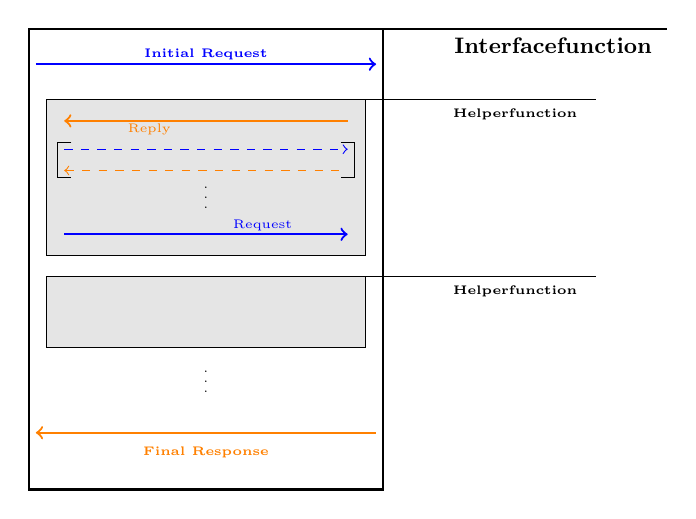
\begin{tikzpicture}[scale=0.9, every node/.style={scale=0.9}]
            % Interfacefunktion
            \draw[thick] (0, 6.5) rectangle (5, 0);
            \draw[thick] (5, 6.5) -- node[below,sloped,pos=0.6]{\small \textbf{Interfacefunction}} (9, 6.5);
            % \node[above] at (1.6, 6.5) {\small \textbf{Interfacefunction}};
            \draw[thick,->,blue] (0.1, 6) -- (4.9, 6) node[above,midway,yshift=-2]{\tiny \textbf{Initial Request}};
            \node[below] at (2.5, 2) {\tiny $\vdots$};
            \draw[thick,<-,orange] (0.1, 0.8) -- (4.9, 0.8) node[below,midway,yshift=-2]{\tiny \textbf{Final Response}};

            \fill[black!10] (0.25, 5.5) rectangle (4.75, 3.3);
            \draw[] (0.25, 5.5) rectangle (4.75, 3.3);
            \draw[] (4.75, 5.5) -- node[below,sloped,pos=0.65]{\tiny \textbf{Helperfunction}} (8, 5.5);
            % \node[above] at (1.1, 5.4) {\tiny \textbf{Helperfunction}};
            \draw[thick,<-,orange] (0.5, 5.2) -- node[below,sloped,pos=0.3,yshift=2.5]{\tiny \text{Reply}} (4.5, 5.2);
            \draw[dashed,->,blue] (0.5, 4.8) -- (4.5, 4.8);
            \draw[dashed,<-,orange] (0.5, 4.5) -- (4.5, 4.5);
            \draw[] (0.6, 4.9) -- (0.4, 4.9) -- (0.4, 4.4) -- (0.6, 4.4);
            \draw[] (4.4, 4.9) -- (4.6, 4.9) -- (4.6, 4.4) -- (4.4, 4.4);
            \node[below] at (2.5, 4.6) {\tiny $\vdots$};
            \draw[thick,->,blue] (0.5, 3.6) -- node[above,sloped,pos=0.7,yshift=-2.5]{\tiny \text{Request}} (4.5, 3.6);

            \fill[black!10] (0.25, 3) rectangle (4.75, 2);
            \draw[] (0.25, 3) rectangle (4.75, 2);
            \draw[] (4.75, 3) -- node[below,sloped,pos=0.65]{\tiny \textbf{Helperfunction}} (8, 3);
            % \node[below] at (2.5, 3) {\tiny $\vdots$};


            % % Request box
            % \draw[thick] (0, 2.5) rectangle (4, 0);
            % \node[below] at (2, 2.5) {$F_\text{id}$};
            % \draw[thick] (0, 2) -- (4, 2);
            % \node[below] at (2, 2) {$F_\text{argument}(1)$};
            % \draw[dashed] (0, 1.35) -- (4, 1.35);
            % \node[below] at (2, 1.53) {$\vdots$};
            % \draw[dashed] (0, 0.7) -- (4, 0.7);
            % \node[below] at (2, 0.7) {$F_\text{argument}(n)$};
            % \draw[decorate, decoration={brace, amplitude=10pt}] (4.1, 2) -- (4.1, 0)
            %     node[midway, right=10pt] {\text{zmsg\_t}};
            % \draw[decorate, decoration={brace, amplitude=3pt}] (4.1, 2.5) -- (4.1, 2)
            %     node[midway, right=12pt] {\text{Integer}};

        \end{tikzpicture}
        % \caption{Die Modularität der Hilfsfunktionen innerhalb einer Interfacefunktion.}
        % \label{fig:help_modular}
    \end{figure}
\end{frame}

\begin{frame}{Logging}
    \vspace{2em}
    \Large
    \begin{enumerate}
        \item dient der verbesserten Nachvollziehbarkeit und Transparenz
        \item lässt sich über die Systemargumente steuern (\enquote{\texttt{-}\texttt{-}log})
        \item schreibt beispielsweise in \texttt{z3rver96485092.probz.log}
    \end{enumerate}
\end{frame}

\begin{frame}[fragile]{Softlock} % verbatim-Umgebungen sind fragil!
    \vspace{2em}
    \inputminted[linenos=false]{c++}{softlocka.cpp}
\end{frame}

\begin{frame}[fragile]{Softlock} % verbatim-Umgebungen sind fragil!
    \vspace{2em}
    \inputminted[linenos=false]{c++}{softlockb.cpp}
\end{frame}

\begin{frame}{Performance-Overhead}
    \begin{center}
        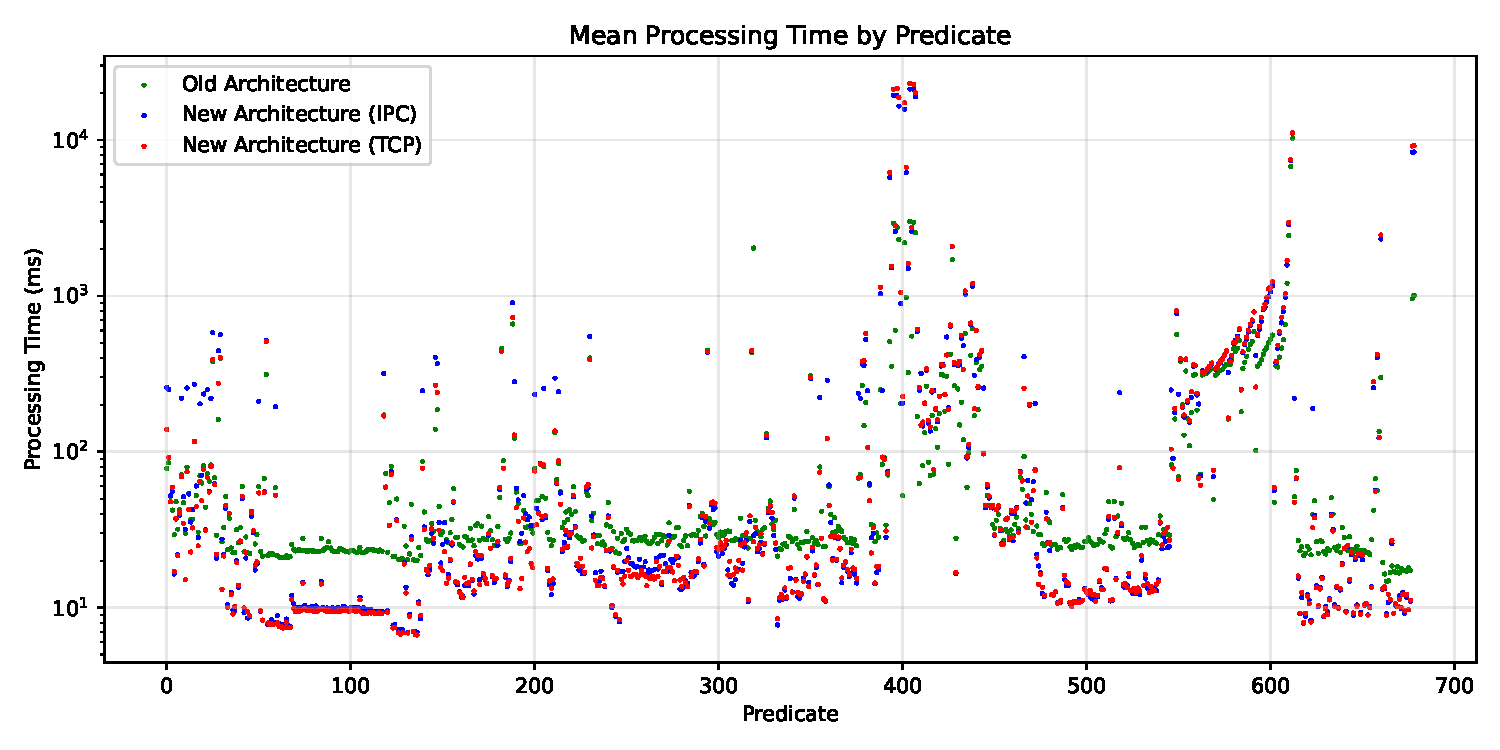
\includegraphics[width=0.85\textwidth]{../Thesis/PerformanceEvaluation/processingtime_small.pdf}
    \end{center}
\end{frame}
